\section*{Parallelization of Matrix-Vector Multiplication and the Power Method}

This report describes the code and result of designing and implementing an algorithm for finding the highest eigenvalue of a matrix, called the Power Method.  The algorithm is designed to run in parallel on N processors to enhance the performance. The Power Method  can easily be described by the following Matlab code 
\lstinputlisting[language=matlab, caption={Power Method algorithm implemented in Matlab (by John R. Gilbert)}]{./code/powermethod.m}

\subsection*{Implementation in the C language}
The code was implemented in C using the MPI library for parallelization. The design of the code was based on first partitioning the matrix operation between the N processors. First a matrix where generated in the function $generatematrix()$. This function generated $\frac{N}{nprocs}$ where nprocs is the number of processors. Further in the code each processors did operations on the same amount of rows. Further, following the algorithm in Listing 1, each processor generated a row column vector of dimension N with 1's in all the entries. Each processor executed the $norm2()$ function on the vector. The parallelization used that helped the performance the most where implemented in the matrix-vector multiplication, in the funciton matVec(). Each processor performed a multiplication with each of the rows and the column vector, producing a column vector of dimension $\frac{N}{nprocs}$. The column vectors from all the processors where gathered in processor 0 using the $MPI\_gather$ library function to form the total matrix-vector product $Ax$. To make the total vector accessible to the other processors, $MPI\_Bcast$ where used. For more details the reader should look at the c-code implementations in functions.c.

\subsection*{Performance and timing}
The c-code where tested on matrices of dimension $N$ where $N$ allways where the quotient $\frac{N}{nprocs}$ always was an integer. The algorithm proved successful and returned the same values as the matlab code, both using the matrix provided in the assignment text, and on an arbitrary matrix. For the timing of the code the dimension matrix dimension $N=2400$ where used, yielding 25.67 seconds of execution time running the code on one processor. The rest of the execution times can be found in Fig. 1 and Table 1. 

\begin{table}
\center
    \begin{tabular}{|l|l|}
        \hline
        nprocs & Execution Time (Seconds) \\ \hline
        1      & 25.67                    \\ 
        2      & 12.95                    \\ 
        4      & 6.47                     \\ 
        8      & 3.41                     \\ 
        16     & 1.97                     \\
        \hline
    \end{tabular}
\end{table}

\begin{figure}[h!] 
 \center 
 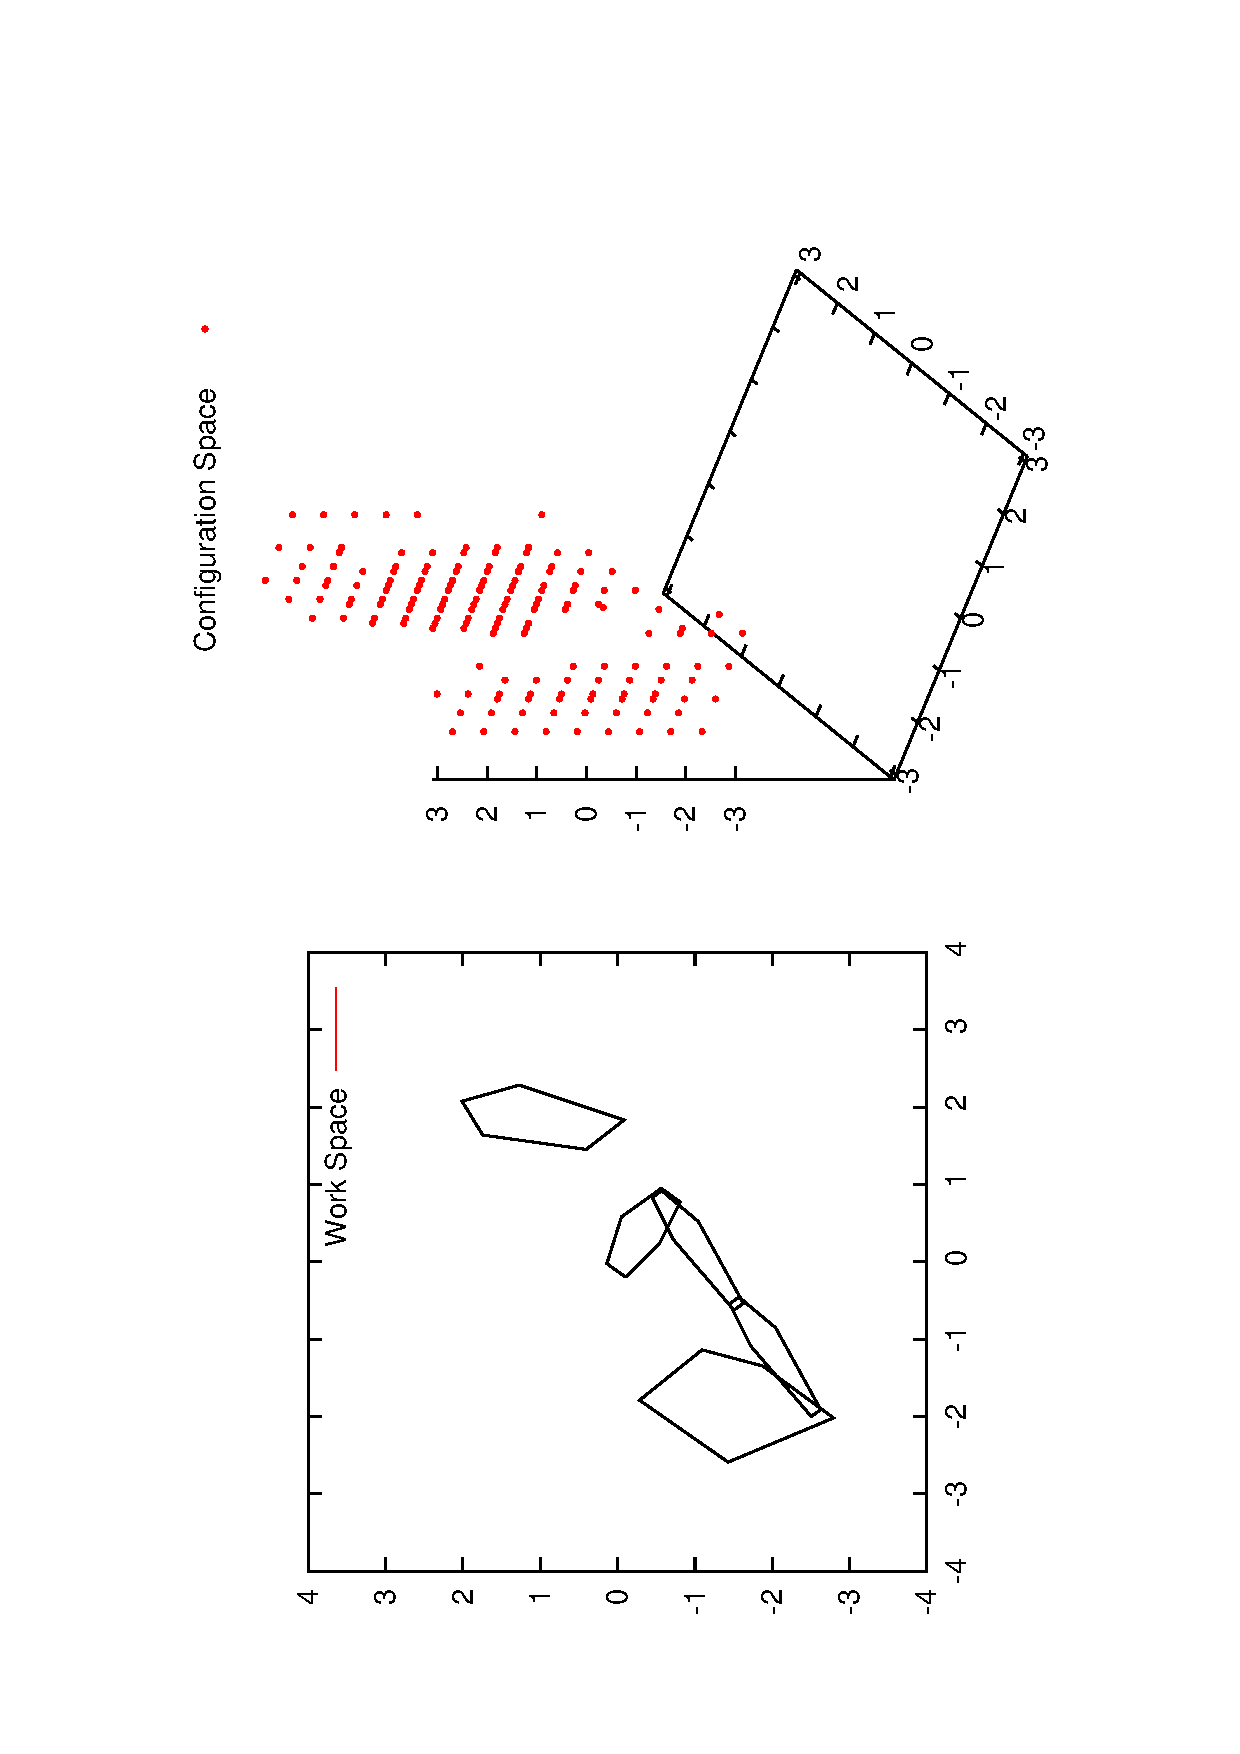
\includegraphics[scale=0.7]{./figures/plot1.pdf}
 \caption{ Plot of the execution times for the code running on 1 to 16 processors \label{fig:plot}}
 \end{figure}

\begin{figure}[h!] 
 \center 
 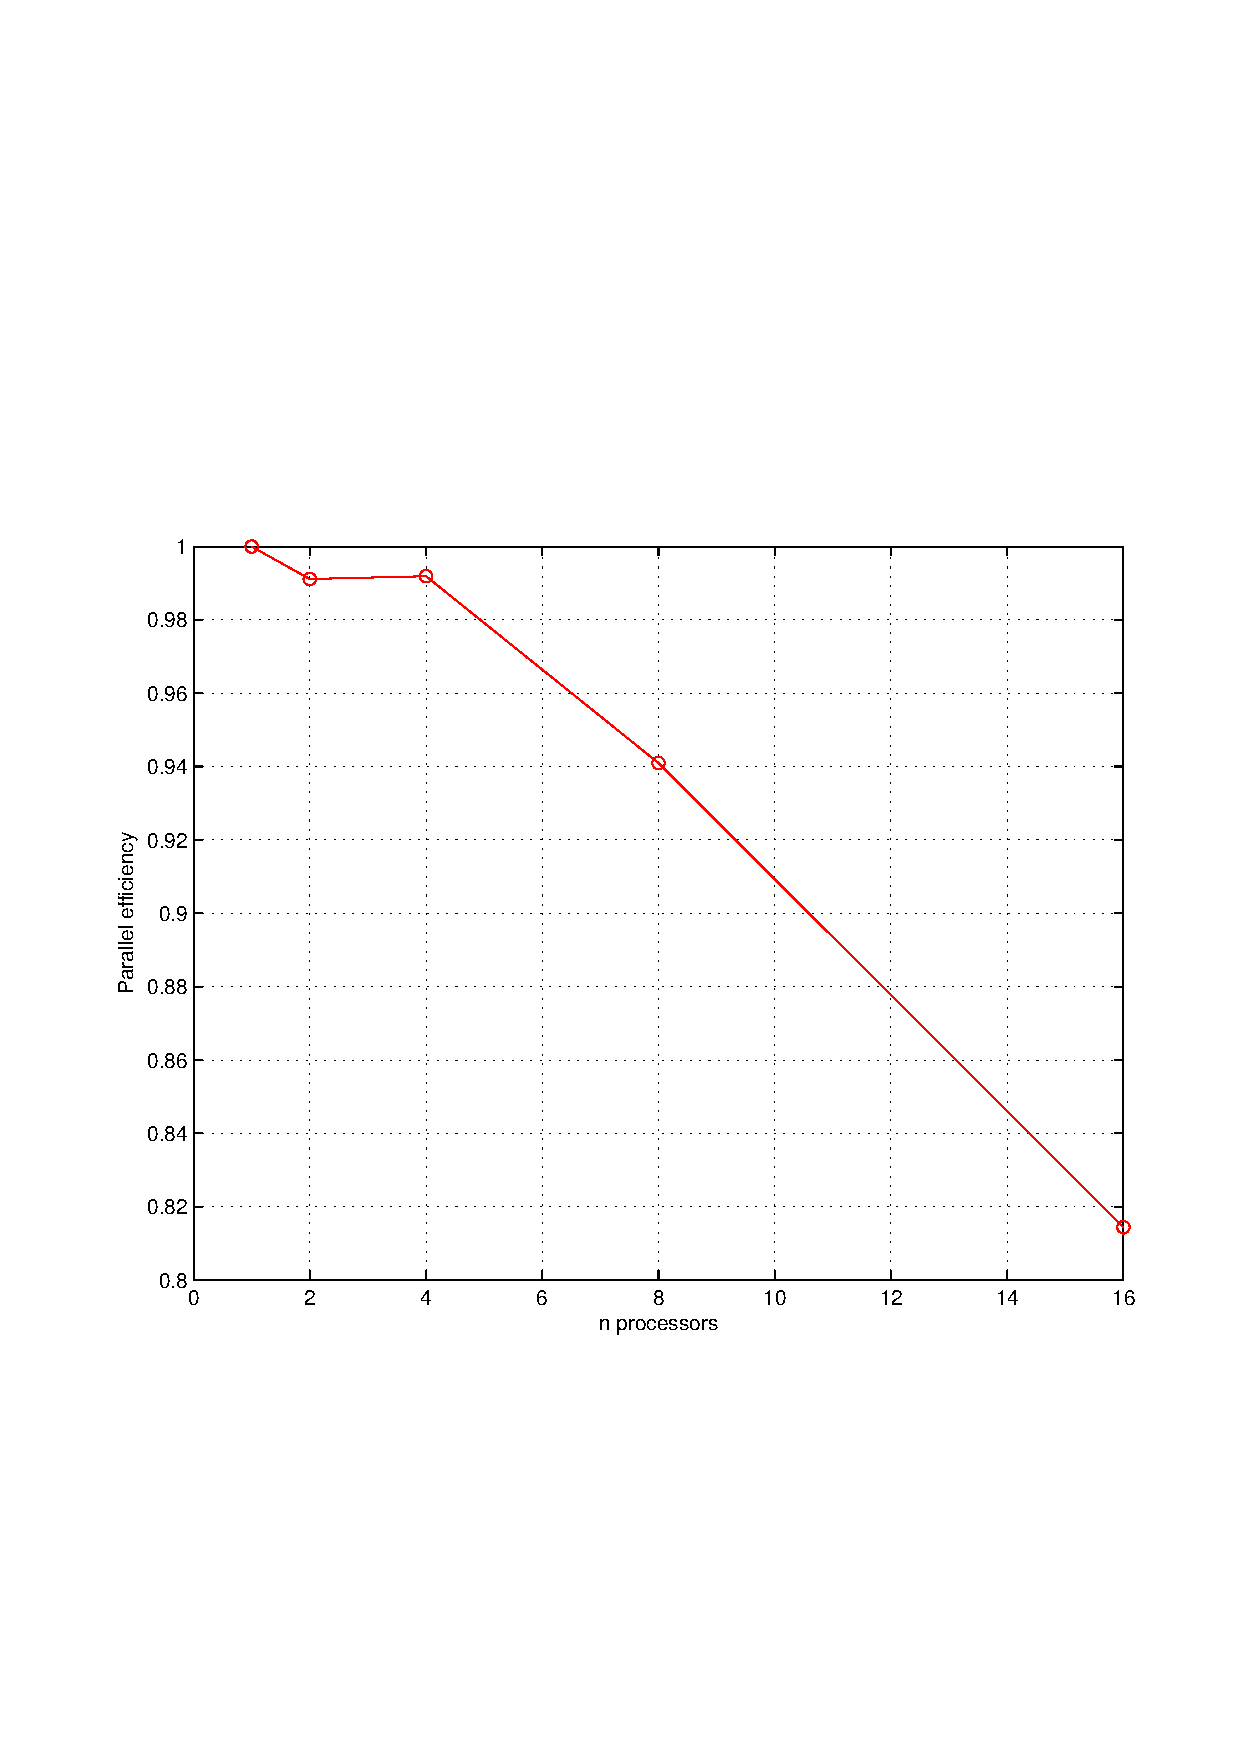
\includegraphics[scale=0.7]{./figures/plot2.pdf}
 \caption{  Plot of the parallel efficiency for the different numbers of processors\label{fig:para}}
 \end{figure}

As we can from Fig. \ref{fig:plot} and Fig. \ref{fig:para} the parallelization of the code worked very well. On matrices with high dimensions the execution time where almost halved when the number of processors where doubled, for a small number of processors. 

\subsection*{Tau Profiling Tool}
The Tau Profiling tool where used to analyze the performance of the code both with a text based interface and with the graphical interface $paraprof$. The program was changed to do only 10 iterations of the main loop. At first the program ran with 4 processors, and than with 16 processors. The results of the generated text profile reports, $pprof$, are in the appendix. From the profile reports it shows that all the processors, except from node 0, have very similar characteristics. They all use most of their time on the initialisation, $MPI\_init$. Beside this it is clear that the $matVec()$ function, who is called in $powerMethod()$, uses a considerable amount of the execution time. Node 0 stands out from the other nodes with the amount of time used on the calls $MPI\_Gather()$ and $MPI\_Bcast$. Node 0, who has to gather data from all the other nodes, uses a lot of time on $MPI\_Gather()$, while all the other nodes uses almost no time on this call. This effect is more reviling with many processors, and is probably one of the main causes why the parallel efficiency goes down with more processors. The call to $MPI\_Bcast$ has the opposite effect. Node 0, who is broadcasting data, uses less time on this call than all the other nodes, which are on the receiving side. 


\subsection*{Conclusion}
The results we got from this assignment was pretty much as expected, but we thought the parallel efficiency was surprisingly good. It was very satisfying seeing the difference between the execution time of the power method with 1 processor versus 16 processors. With many processors, the synchronisation with $MPI\_Gather()$ and $MPI\_Bcast$ takes more time than the actual multiplication done in $matVec()$, and leads to less parallel efficiency. This is no surprise since moving data takes time.\\
From the figures in $parafrof$ it was very quick and easy to get a first overview over the execution time for the different MPI functions. It was also easy to compare the running times between the different processors. From the text profile report, $pprof$, we got more detailed information.

 
\begin{figure}[h!] 
 \center 
 \subfloat[]{ 
 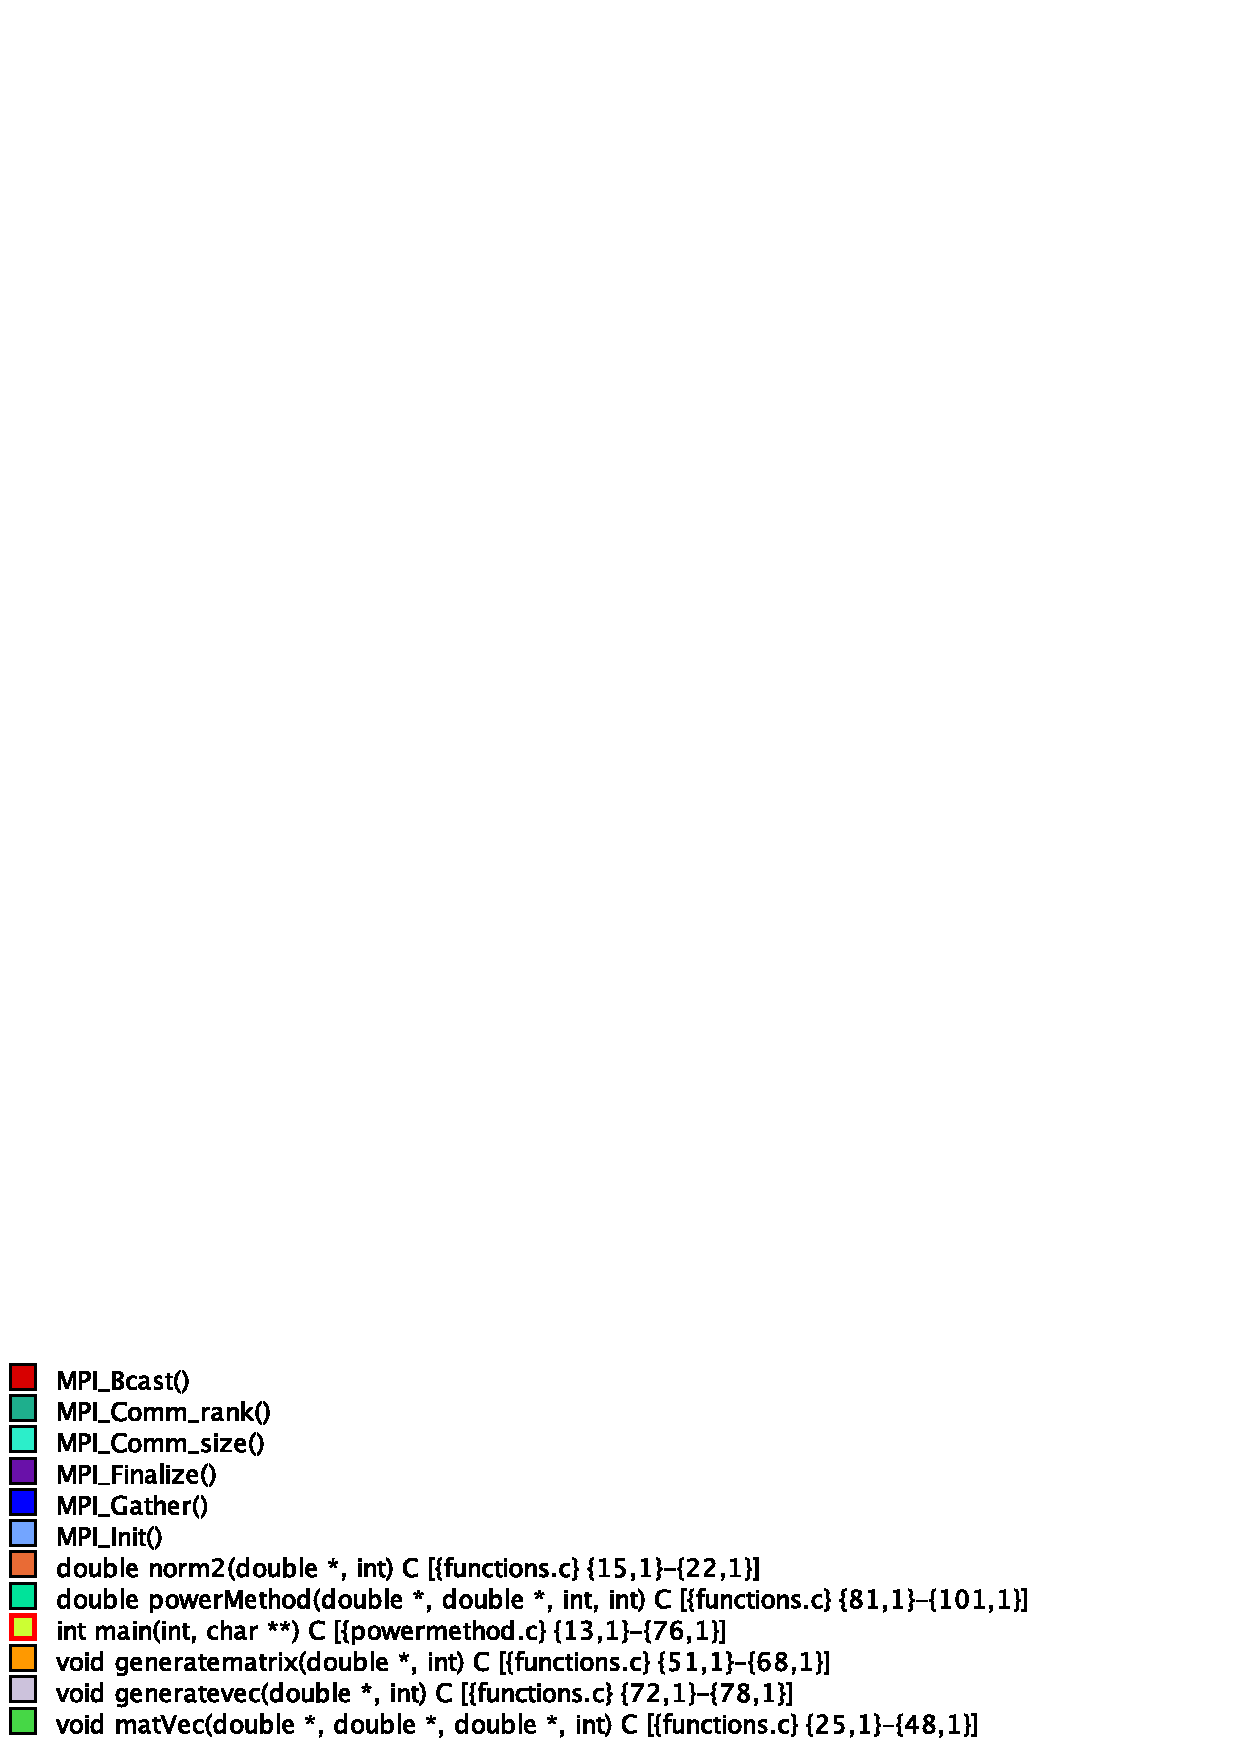
\includegraphics[scale=0.4]{./figures/legend_16.pdf} } \\
 \subfloat[]{ 
 \includegraphics[scale=0.3]{./figures/paraprof_pic_16.pdf} }
 \caption{ The figure shows the execution time for the different MPI functions running on the different processors \label{fig:}}
 \end{figure}


\clearpage



\includepdf[pages=1]{side1.pdf}
\includepdf[pages=2-8]{log.pdf}



















